\chapter{Analysis of Transmission line problems}
This chapter deals with solving problems based on the theory developed so far. We will first solve problems analytically and then use the graphical method to solve some more problems.

\bigskip

\bigskip

\bigskip
\section{\textbf{Analytical method of analysis}}
\begin{example}
	A loss-less transmission line has 75$\Omega$ characteristic impedance. The line is terminated in a load impedance of $50-j100\Omega$. The maximum voltage measured on the line is 100v. Find the maximum and minimum current, and the minimum voltage on the line. At what distance from the load are the voltage and the current maximum?
\end{example}
\begin{center}
	\underline{\textbf{\large Solution}}
\end{center}
Given,
$Z_{0}=75\Omega,$
$Z_{L}=50-j100\Omega,$
$|V|_{max}=100V,$

\begin{itemize}
	\item 
	The first step is to calculate the reflection coefficient.
	\begin{align*}
		\Gamma_{L}=\frac{Z_{L}-Z_{0}}{Z_{L}+Z_{0}}\\\\
	=\frac{50-j100-75}{50-j100+75}=0.64\angle-65.3^{0} \\\\
	|\Gamma_{L}|=0.64,\\\\ \phi_{L}=-65.3^{0}
	\end{align*}
	Since we are told that the line is lossless, then the reflection coefficient will remain constant throughout the line.
	
	\item We know that the maximum voltage which we will see on the line $|V|_{max}=|V^{+}|[1+|\Gamma_{L}|]$, and we are given $|V|_{max}$, we also know now the modulus of reflection coefficient, so we can find out the magnitude of the incident wave $|V^+|$.\\
	So,
	\begin{align*}
	100=|V^{+}|[1+0.64]\\\\
	|V^{+}|=\frac{100}{1.64}=60.8V
	\end{align*}
	
	\item We know from previous analysis that the maximum current $|I|_{max}$ seen on the transmission line is $\frac{|V|_{max}}{Z_0}$.\\
	So,
	\begin{align*}
	 |I|_{max}=\frac{|V|_{max}}{Z_0}\\\\
	 =\frac{100}{75}=1.33A
	\end{align*}
	
	\item From the previous chapters , we established that $|I|_{min}=\frac{|V^{+}|}{Z_0}(1-|\Gamma_{L}|)$.
	\begin{align*}
	|I|_{min}=\frac{60.8}{75}(1-0.64)\\\\
	         =0.29A
	\end{align*}
	
	\item Then we can find out the minimum voltage which is,	
	\begin{align*}
	|V|_{min}=Z_0|I|_{min}\\\\
	         =75\times0.29=21.88V
	\end{align*}
	
	\item Lastly, the question request that we locate the distance from the load where the current and voltage are maximum. Let us note that when the two traveling waves have a constructive interference, we have a voltage maximum which corresponds to the current minimum. Also, when two traveling waves have a destructive interference, we have a voltage minimum which corresponds to the current maximum.\\
	The phase difference between the forward and the backward wave is given by $\phi_{L}-2\beta l$. Where $\phi_L$ is the phase angle of the reflected wave.
	
	\item
	If $\phi_{L}-2\beta l$ is even multiples of $\pi$, the two waves will  have a constructive interference and the voltage will be maximum. Let us recall from chapter 5 that when $\phi_{L}-2\beta l$ is odd multiples of $\pi$, it has a destructive interference and a voltage minimal will be observed. So mathematically, voltage maximum occurs at $\phi_{L}-2\beta l= \pm2m\pi$, where m is an integer quantity.
	
	\item
	NOTE: The $2m\pi$ is as a result of the fact that from one voltage maximum, you would have to move a complete revolution before getting to another voltage maximum. To get a positive length, l, we will move towards the generator(clockwise) which implies negative angle $2m\pi$.
    \begin{align*}
    \phi_{L}-2\beta l_{max}=-2m\pi\\\\
    2\beta l_{max}= \phi_{L}+2m\pi
    \end{align*}
    But, $\beta = \frac{2\pi}{\lambda}$
    \begin{align*}
    2 \times \frac{2\pi}{\lambda}\times l_{max}= \phi_{L}+2m\pi\\\\
    l_{max}=\frac{(\phi_L + 2m\pi)\lambda}{4\pi}
    \end{align*}
    We know $\phi_{L}=-65.3^{0}=-1.14rad$
    \begin{align*}
    l_{max}=\frac{(-1.14 + 2m\pi)\lambda}{4\pi}
    \end{align*}
	using values of m = 1,2,3...\\
	$l_{max}=0.41\lambda , 0.91\lambda, 1.41\lambda$ and so on.
	
	\item
	To find the current maximum, we have to understand that the current maximum occurs at a point where the voltage is minimum and the current minimum occurs at a point where the voltage is maximum. The voltage maximum and voltage minimum are shifted by a distance of $\frac{\lambda}{4}$. Simply put, the current maximum and voltage maximum are shifted by a distance of $\frac{\lambda}{4}$.\\
	
	So, current maximum is at $l_{max}(voltage)\pm \frac{\lambda}{4}$. Using the negative and positive sign will both give correct answers. Here, we will use the negative sign, i.e $l_{max}-\frac{\lambda}{4}$.\\
	
	So $|I|_{max}$ occurs at $0.16\lambda , 0.66\lambda , 1.16\lambda$ and so on.
	\item Using the basic equations which we have for the transmission line, the steps we followed are: we found the reflection coefficient, got the relationship of the voltage and current, wrote down the simple voltage and current expressions on the transmission line, then , substituting for the values of the reflection coefficient-its magnitude and its phase-we were able to calculate the maximum and minimum current and voltage on the transmission line. Also, we found the locations of which the voltage or current were maximum or minimum. This is one of the problems which we will be asked to solve in real life. Normally, the line is terminated at an unknown impedance and we are supposed to find out where the voltage will be maximum and so on and so forth.
\end{itemize}

\begin{example}
	A $50\Omega$ transmission line is connected to a parallel combination of a $100\Omega$ resistance and a 1nF capacitance. Find the VSWR on the line at a frequency of 2MHZ. Also, find the maximum and minimum resistance seen on the line.
\end{example}

\begin{figure}[h]
	\centering
	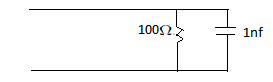
\includegraphics[width=\linewidth]{d1}

	\caption{Circuit diagram}
\end{figure}

\begin{center}
	\textbf{\underline{{\large Solution}}}
\end{center}

\begin{itemize}
	\item First, we will find out the complete impedance for the parallel combination of the resistor and capacitor, given as $Z_{L}=R||X_c$\\
	$X_c =\frac{1}{j\omega C}$
	\begin{center}
		$Z_L=\frac{R \times X_c}{R + X_c}$

	\end{center}
	\begin{align*}
	=(R\times\frac{1}{j\omega C})/(\frac{j\omega RC + 1}{j\omega C})\\\\
	=\frac{R}{j\omega C} \times \frac{j \omega C}{j\omega RC + 1}\\\\
	=\frac{R}{j\omega RC + 1}
	\end{align*}
	Given $f=2MH_{z}$,\\
	$\omega = 2\pi f$\\
	$\omega= 2\pi \times 2 \times 10^{6}$\\
	$=1.256\times 10^{7}$ rad/s
    \begin{align*}
    	Z_{L}=\frac{100}{1 + j1.2566}\\\\
     = 38.77-j48.7\Omega = 62.3\angle-51.5^{0}\Omega
    \end{align*}
    
    \item Next, we find the refection coefficient.\\
	Reflection coefficient at load point, $\Gamma_{L}=\frac{Z_{L}-Z_{0}}{Z_{L}+Z_{0}}$
	\begin{align*}
	\Gamma_{L} = \frac{38.77-j48.7-50}{38.77-j48.7+50}
	=0.13-j0.47 = 0.5\angle-74.23^0
	\end{align*}
	
	We get $|\Gamma_{L}|=0.5$ and $\phi_L = -74.23^0$
	
	\item Now, we know the reflection coefficient, we can find out VSWR, $\rho$, given as;
    \begin{align*}
    	\rho=\frac{1 + |\Gamma_{L}|}{1-|\Gamma_{L}|}\\\\
    	=\frac{1+0.5}{1-0.5} = 3
    \end{align*}
     
     \item $R_{max}$ and $R_{min}$ can be calculated from these relationships:
     $R_{max} = Z_0\rho$ and $R_{min} = \frac{Z_0}{\rho}$ such that
     \begin{align*}
     R_{max} = 50 \times 3 = 150\Omega\\\\
     R_{min} = \frac{50}{3} = 16.67\Omega
     \end{align*}
\end{itemize}

\section{Graphical method of analysis}
\begin{example}
	Now, we will try to solve some of the problems by using the smith chart, i.e the graphical method.\\
	We are going to first identify some specific points on the smith chart.
	
	A. 50+j75$\Omega$
	
	B. 10+j0$\Omega$
	
	C. 0-j80$\Omega$
	
	D. $\Gamma=0.3\angle60^{0}$
	
	E. VSWR circle for $\rho=2.5$
	
	F. $R_{min}$ on $\rho$ = 1.5  circle
	
	Take characteristic impedance, $Z_{0}$ = 50$\Omega$
\end{example}

\begin{center}
	\textbf{\underline{\large Solution}}
\end{center}

\begin{figure}
	\includegraphics[width=1\linewidth]{"Smith chart"}
\end{figure}
\begin{itemize}
	\item All impedances seen on the smith chart are normalized impedances. Therefore, for impedance A, B, C, we will first normalize these points with the characteristic impedance.\\
   \begin{align*}
   \bar{A}=\frac{A}{Z_{0}}\\
   \bar{A}=\frac{50 + j75}{50}\\
   \bar{A}=1+j1.5\\
   \bar{B}=\frac{B}{Z_{0}}\\
   \bar{B}= \frac{10 + j0}{50}\\
   \bar{B}=0.2+j0\\
   \bar{C}=\frac{C}{Z_{0}}\\
   \bar{C}= \frac{0 - j80}{50}\\
   \bar{C}=0-j1.6
   \end{align*}
	
	\item 
	To locate point A on the smith chart, we first identify the constant resistance circle of r = 1.0 . It is the circle which passes through the center of the smith chart from the right hand side. Next, we go to the reactive part which is the 1.5 value. Circles above the horizontal line passing through the center are the inductive reactance, while the arcs below the line are the capacitive reactance. Since the value 1.5 is positive, it should be the constant inductive reactance circle(i.e arcs above the center horizontal line). Where the circle and arc intersect is point A, which represents the normalized impedance, 1 + j1.5. Same applies for B and C.
	
	\item 
	For point D which is the reflection coefficient, the approach is quite different. First, we measure the length of the diameter for constant resistance circle r = 1.0. When measured, we will get a value of 7.6cm. When scaled down by multiplying it with the value of the reflection coefficient which is 0.3, we will get a value, 2.28cm. Draw a circle of radius 2.28cm from the origin on the smith chart. Along the circumference of one of the outer circles where it shows (ANGLE OF REFLECTION COEFFICIENT IN DEGREES) we will move $60^0$ anticlockwise. Then draw a straight line through the center to the point $60^0$ on the smith chart. Where it intersects the circle drawn, is a point  which is $\Gamma = 0.3\angle60^{0}$ on the smith chart.
	
	\item 
   To locate point E, we will place a compass on the center of the smith chart. Locate the point that reads r = 2.5 along the horizontal line on the smith chart. The VSWR circle of 2.5 is drawn through that point.
	
	\item 
   To locate point F, first, we repeat the process used to draw $\rho = 2.5$. The rightmost side along the circle where the horizontal line intersects the VSWR circle is the normalized $R_{max}$ and the leftmost side is the normalized $R_{min}$. So at the leftmost side of the VSWR circle we locate the normalized $R_{min}$. Multiply the value of the normalized $R_{min}$ by the characteristic impedance$(\bar{R}_{min} = \frac{R_{min}}{Z_0})$ to get the value of the minimum resistance.
   	\begin{align*}
   	R_{min}  = 0.75 \times 50 = 37.5\Omega
   	\end{align*}
\end{itemize}

\begin{example}
	A 50$\Omega$ line is terminated in a load impedance  $25+j35\Omega$. With the help of the smith chart, find 
	
	(i)Reflection coefficient in cartesian and polar form,
	
	(ii)Reflection coefficient and impedance at a distance of $0.2\lambda$ from the load end of the line.
	
	(iii)VSWR on the line.
\end{example}

\begin{center}
	\textbf{\underline{\large Solution}}
\end{center}
We are given $Z_{L}=25+j35\Omega$ and $Z_{0}=50\Omega$

\begin{center}
	\includegraphics[width=1\linewidth]{"Smith chart 1"}
\end{center}


\begin{itemize}
	\item First, we normalize the load impedance
    \begin{align*}
    \bar{Z_{L}}=\frac{25+j35}{50}\\\\
    =0.5+j0.7
    \end{align*}
	
	\item
	We mark this point on the smith chart as shown in the fig. above.
	
	\item
	To get the reflection coefficient, we draw a circle from the center on the smith chart through the normalized impedance point, A. The distance between point A and the center gives the magnitude of the reflection coefficient; the distance is read from the scale for reflection coefficient E or I at the bottom of the smith chart page( \underline{Note}: This method is different from that used in the previous problem and both methods are correct). From which we get
	\begin{align*}
	|\Gamma_{L}| = 0.52
	\end{align*}
	
	\item
	Also, for the angle $\phi_{L}$, draw a straight line from the center through point A to the outermost circle as shown. From the angle of reflection coefficient scale, read the angle it makes with the positive x-axis. That gives you the angle of the reflection coefficient in polar form.\\
	The value obtained is $0.52\angle100^{0}$(polar form). To get the value in cartesian form,
	\begin{center}
		$0.52\angle100^0 = 0.52e^{j100} = 0.52{\cos100 + j\sin100}$
	\end{center}
	 Which gives us
	 \begin{align*}
	 \Gamma_{L} = -0.09+j0.512
	 \end{align*}
	
	\item 
	The next step is to get the reflection coefficient at a distance of $0.2\lambda$ from the load point.\\
	First, we identify the scale on the outermost circle that shows (WAVELENGTH TOWARDS GENERATOR). The value measured at point A is $0.11\lambda$. To move a distance $0.2\lambda$ towards the generator means to move clockwise along the scale. Similarly, moving towards the load on the smith chart means to move in the anticlockwise direction along the scale which shows WAVELENGTH TOWARDS THE LOAD. We mark this point as B, which is 0.11$\lambda + 0.2\lambda$= $0.31\lambda$. Draw a straight line from 0.31$\lambda$ towards the center of the smith chart. Where it intercepts the VSWR circle is the point marked P which is the point of the reflection coefficient moved $0.2\lambda$ towards the generator. It should be noted that the value of the reflection coefficient remains the same as we assume the line is a lossless line, but its phase changes, which can be measured by using the angle of reflection coefficient scale, with the positive x-axis as your reference and measuring the angle anticlockwise towards the point of consideration. 
	
	\begin{center}
		$\Gamma$ at $0.2\lambda$ from the load  = $0.52\angle316^{0}$
	\end{center}
	
	\item
	To find the normalized impedance at point P, we check for the constant resistance and reactance circle  it corresponds with. The value gotten is 
	\begin{center}
		$\bar{Z}=1.4-j1.37$
	\end{center}
	However, we have to convert to impedance value as shown
    \begin{align*}
    Z=Z_{0}\times\bar{Z}\\\\
    Z= 50(1.4-j1.37) = 70-j68.5\Omega
    \end{align*}
	
	\item
	The VSWR value $\rho$ is obtained by reading the value shown at the rightmost side of the VSWR circle.
	
    \begin{center}
    		VSWR, $\rho = 3.8$
    \end{center}
	
	\item 
	Hence, without doing any gross calculation, we were able to derive all these from the smith chart. The use of smith chart makes calculation for Transmission line extremely simple. If we had gone through the impedance transformation analytically, this would have been quite tedious to do.
\end{itemize}

\begin{example}
	A line is terminated in a normalized admittance $0.2-j0.5$. Find the location of the voltage maximum from the load  end. Also find the reflection coefficient , normalized admittance and normalized impedance at a distance 0.12$\lambda$ from the load.
\end{example}

\begin{center}
	\textbf{\underline{\large Solution}}
\end{center}

\begin{center}
	\centering
	\includegraphics[width=1\linewidth]{"smith chart 3"}
\end{center}

\begin{itemize}
	\item Now, in this problem we shall be dealing with admittances instead of impedances which we are used to. The admittance we are given here is already normalized, so we can go to the smith chart and mark it out exactly.
	\begin{center}
			$\bar{Y} = 0.2 - j0.5$
	\end{center}
	
	\item 
	The point is marked on the smith chart corresponding to the normalized admittance. Next, we draw a circle from the center of the smith chart through that point $\bar{Y}_L$.
	
	\item 
	Next we need to find the location of the voltage maximum from the load end. However, for the admittance smith chart, the voltage maximum will now lie on the leftmost side of the VSWR circle of the smith chart. This point is denoted by $V_{max}$ on the smith chart above. The distance between  $\bar{Y}_L$ and $V_{max}$ on the smith chart is the length to be moved towards the generator to get to the maximum voltage point. Recall that we move clockwise when moving towards the generator. The constant VSWR circle is shown on the smith chart.
	
	\item
	The next thing we are asked to find is the reflection coefficient, normalized admittance and the normalized impedance at a distance of $0.12\lambda$.
	
	\begin{itemize}
		\item 
	    As explained in the previous example, the corresponding wavelength for the normalized admittance, $\bar{Y}_L$ is $0.424\lambda$. Moving a distance of $0.12\lambda$ towards the generator is 
	    \begin{center}
	    	$0.424\lambda$ + $0.12\lambda$= $0.544\lambda$
	    \end{center}
		
		\item
		But the highest value on the wavelength scale is $0.5\lambda$ so the value on the scale which corresponds to $0.544\lambda$ is $0.044\lambda\footnote{0.544-0.5}$. Next we draw a line through that point to the center of the smith chart. The point where the line drawn intercepts the VSWR circle is point $\bar{Y}$. The value of normalized admittance is given at that point as:
		
		  \begin{center}
		  	$\bar{Y} = 0.18 + j0.28$
		  \end{center}
	      
	      \item 
		To get the normalized impedance at a distance of $0.12\lambda$ from the load point, we know from previous studies that the normalized impedance inverts itself every $\frac{\lambda}{4}$. Also, the normalized admittance is the reciprocal(inverse) of the normalized impedance. Therefore, to get the normalized impedance on the smith chart, we have to move a distance of $\frac{\lambda}{4}$. With this idea established, draw a straight line from the normalized admittance, $\bar{Y}$ through the center such that it divides the smith chart into halves. We  mark this point as $\bar{Z}$ which is $180^{0}$ from the point $\bar{Y}$.
		
		\begin{center}
			$\bar{Z} = 1.6 - j2.6$
		\end{center}
		
		\item 
		Finally, we need to measure the reflection coefficient. As stated earlier, we measure the distance between the center and $\bar{Z}$ with a pair of divider preferably and read its value on the scale at the bottom of the smith chart page. Or alternatively, the distance measured is divided with the distance measured for the diameter of the r = 1.0 circle. Both answers are the same.
		
		\item 
	   What  we did earlier, only gives the magnitude of $\Gamma_{L}$. For the angle $\phi_L$, it is measured at $\bar{Z}$, from the positive x-axis. From the Smith Chart above the angle measured is negative along the angle of reflection coefficient because it is measured clockwise, and it reads $-32^0$ which is $328^0$ measured from the positive x-axis. So,
		
		\begin{center}
			$\Gamma = 0.7\angle328^{0}$
		\end{center}
	\end{itemize}
      \item 
		All these demonstrate is the effectiveness of the smith chart in moving from impedance to admittance and vice versa. We switch from impedance to admittance by diagonally switching between them on the smith chart.
		
		\item 
		At the load point, $\bar{Y_{L}}$, if we go diagonally opposite, we get $\bar{Z_{L}}$. So basically, it helps us invert complex number. 
\end{itemize}


